\Article{17}
\begin{center}\emph{Theory of the biquadratic residue} $1+i$.\end{center}
The modulus must have no divisor in common with the residue. We therefore assume that one of the numbers $a$ and $b$ is even and the other odd. The following diagram shows the distribution of the proper primitive residues into the four classes:
\begin{center}\resizebox{.90\textwidth}{!}{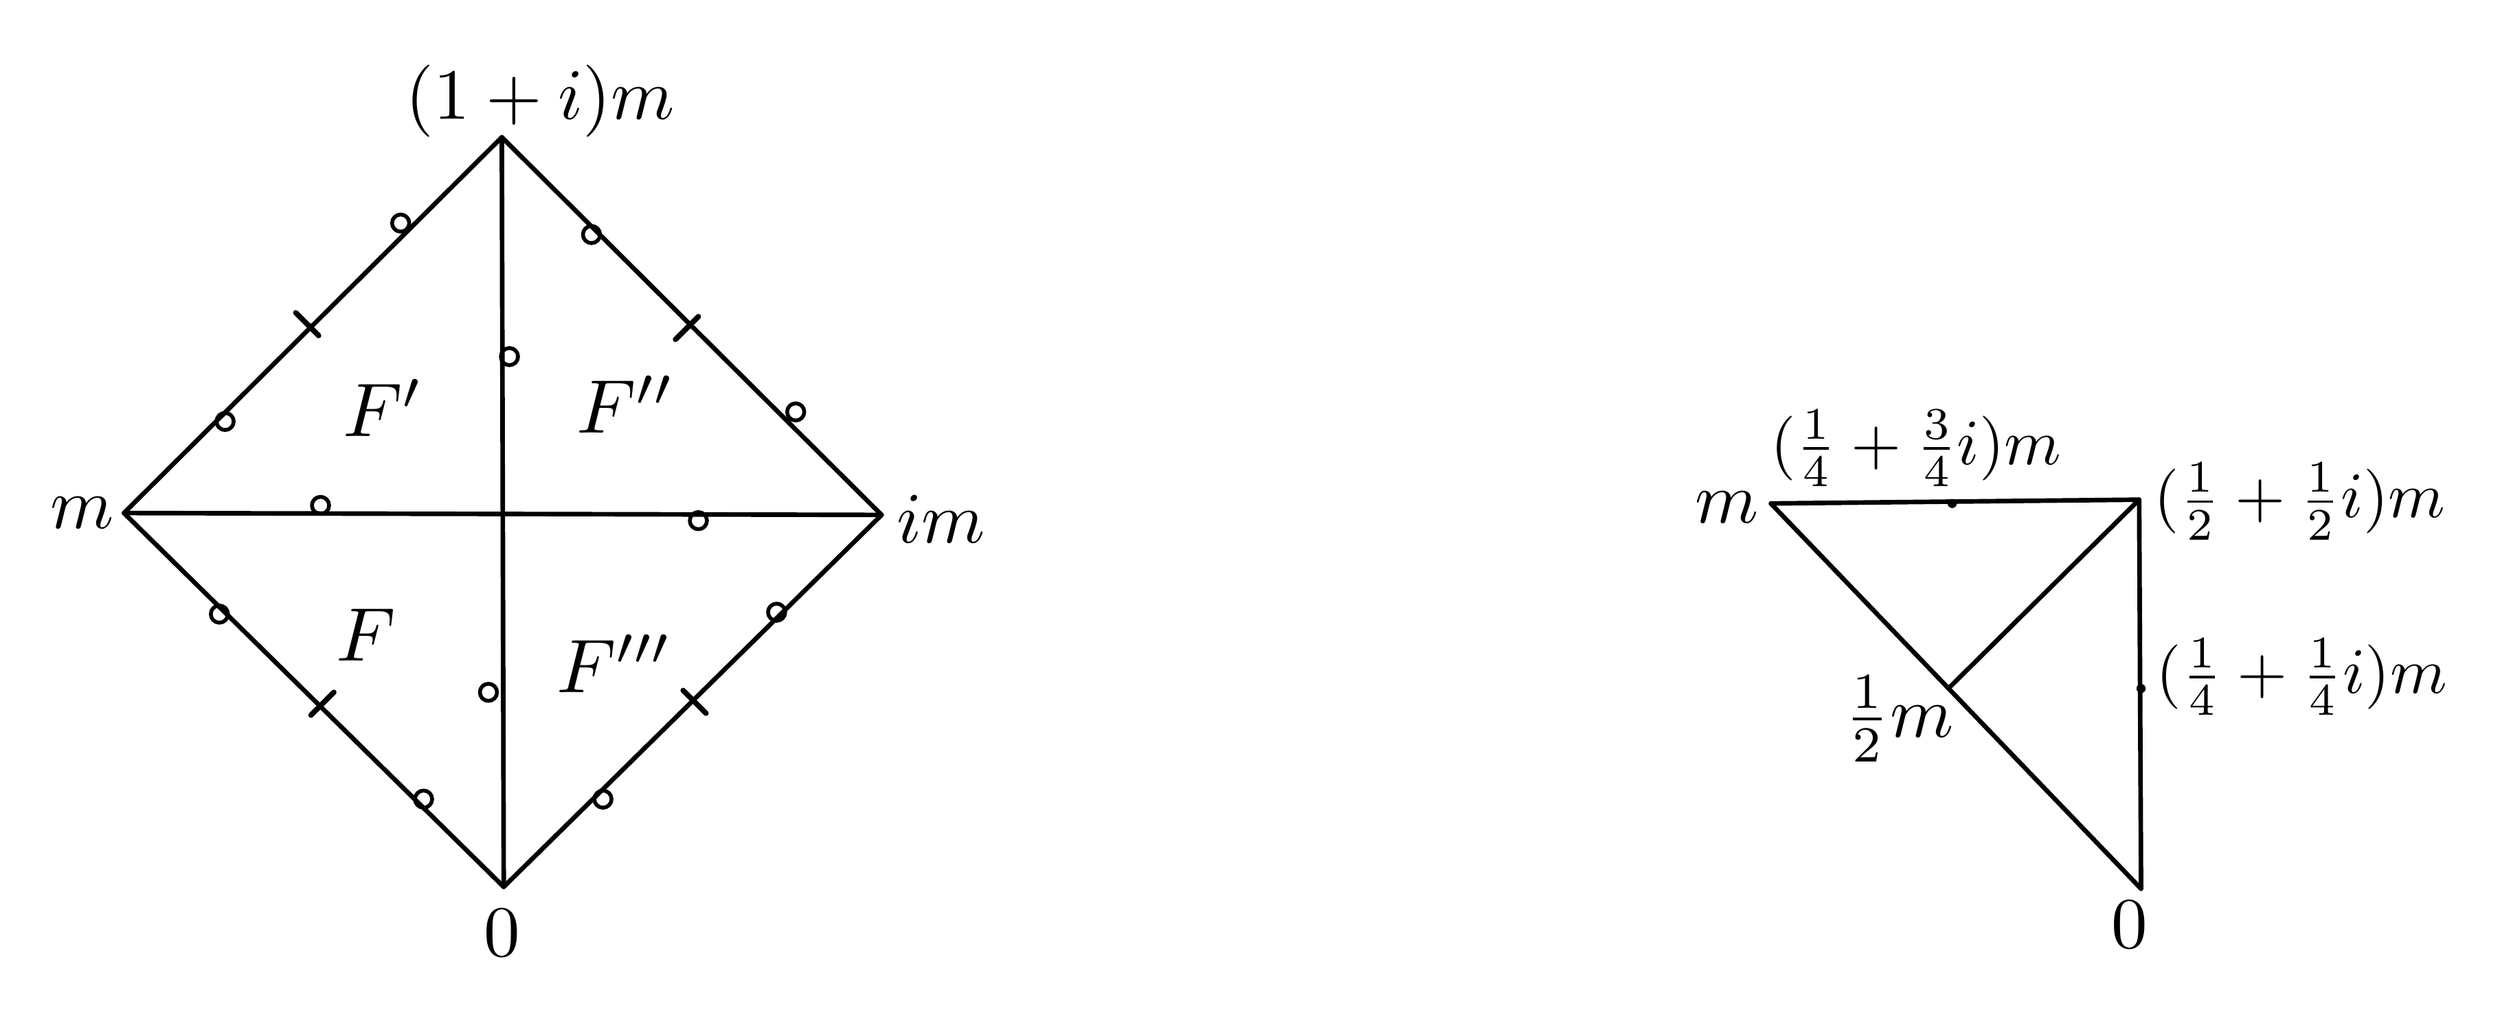
\begin{tikzpicture}[x=1bp,y=-1bp,line cap=round,line join=round]
\path[use as bounding box] (0,0) rectangle (1290,520);
\begin{pgfinterruptboundingbox}
\draw[line width=2.4bp] (55,259) -- (253,62) -- (452,260) -- (254,455) -- cycle;
\draw[line width=2.4bp] (253,62) -- (254,455);
\draw[line width=2.4bp] (55,259) -- (452,260);
\draw[line width=2bp] (108,211) circle[radius=4.5bp];
\draw[line width=2bp] (200,107) circle[radius=4.5bp];
\draw[line width=2bp] (300,113) circle[radius=4.5bp];
\draw[line width=2bp] (407,206) circle[radius=4.5bp];
\draw[line width=2bp] (105,312) circle[radius=4.5bp];
\draw[line width=2bp] (212,409) circle[radius=4.5bp];
\draw[line width=2bp] (397,311) circle[radius=4.5bp];
\draw[line width=2bp] (306,409) circle[radius=4.5bp];
\draw[line width=2bp] (158,255) circle[radius=4.5bp];
\draw[line width=2bp] (356,263) circle[radius=4.5bp];
\draw[line width=2bp] (257,177) circle[radius=4.5bp];
\draw[line width=2bp] (246,353) circle[radius=4.5bp];
\draw[line width=2.8bp] (145,154) -- (157,166);
\draw[line width=2.8bp] (344,168) -- (356,156);
\draw[line width=2.8bp] (153,365) -- (165,353);
\draw[line width=2.8bp] (348,352) -- (360,364);
\node[inner sep=0pt,outer sep=0pt,anchor=center] at (191,204) {\scalebox{4}{\ensuremath{F'}}};
\node[inner sep=0pt,outer sep=0pt,anchor=center] at (318,202) {\scalebox{4}{\ensuremath{F''}}};
\node[inner sep=0pt,outer sep=0pt,anchor=center] at (182,323) {\scalebox{4}{\ensuremath{F}}};
\node[inner sep=0pt,outer sep=0pt,anchor=center] at (312,338) {\scalebox{4}{\ensuremath{F'''}}};
\node[inner sep=0pt,outer sep=0pt,anchor=center] at (33,259) {\scalebox{3.8}{\ensuremath{m}}};
\node[inner sep=0pt,outer sep=0pt,anchor=center] at (273,43) {\scalebox{3.8}{\ensuremath{(1+i)m}}};
\node[inner sep=0pt,outer sep=0pt,anchor=center] at (483,262) {\scalebox{3.8}{\ensuremath{im}}};
\node[inner sep=0pt,outer sep=0pt,anchor=center] at (253,479) {\scalebox{3.8}{\ensuremath{0}}};
\draw[line width=2.4bp] (918,254) -- (1111,252) -- (1112,456) -- cycle;
\draw[line width=2.4bp] (1011,351) -- (1111,252);
\fill (1013,254) circle[radius=2.4bp];
\fill (1112,351) circle[radius=2.4bp];
\node[inner sep=0pt,outer sep=0pt,anchor=center] at (895,256) {\scalebox{3.8}{\ensuremath{m}}};
\node[inner sep=0pt,outer sep=0pt,anchor=center] at (994,225) {\scalebox{3.4}{\ensuremath{(\frac14+\frac34 i)m}}};
\node[inner sep=0pt,outer sep=0pt,anchor=west] at (1119,253) {\scalebox{3.4}{\ensuremath{(\frac12+\frac12 i)m}}};
\node[inner sep=0pt,outer sep=0pt,anchor=center] at (985,367) {\scalebox{3.8}{\ensuremath{\frac12 m}}};
\node[inner sep=0pt,outer sep=0pt,anchor=west] at (1120,345) {\scalebox{3.4}{\ensuremath{(\frac14+\frac14 i)m}}};
\node[inner sep=0pt,outer sep=0pt,anchor=center] at (1106,475) {\scalebox{3.8}{\ensuremath{0}}};
\end{pgfinterruptboundingbox}
\end{tikzpicture}
}\end{center}

Count towards $n$ all numbers on
\[
\text{the line }0\ldots\tfrac12m\qquad\text{number }=g
\]
Towards $n'$, all numbers on
\[
\text{the line }0\ldots(\tfrac14+\tfrac14i)m\qquad\text{number }=g'
\]
Towards $n''$, all numbers inside
\[
\text{the triangle }\tfrac12m,m,(\tfrac12+\tfrac12i)m\qquad\text{number }=h
\]
Towards $n'''$, all numbers inside
\[
\text{the triangle }0,\tfrac12m,(\tfrac12+\tfrac12i)m\qquad\text{number }=h'
\]
and also all numbers on
\[
\text{the line }(\tfrac14+\tfrac14i)m\dotstwo(\tfrac12+\tfrac12i)m\qquad\text{number }=g''
\]

We always have $g'+g''=g$, $aa+bb=p$, $\frac14(p-1)=g+g'+g''+h+h'$. The decident is therefore
\SourceLeaf{329}

\[
D=S(0_{(+)},\tfrac12m,(\tfrac12+\tfrac12i)m_{(-)})+\tfrac12(p-1)+2g''
\]

Now suppose that, for the modulus $m+1+i$,
\[
\begin{array}{clc}
g&\text{changes to}&G\\
g'&&G'\\
g''&&G''\\
h&&H\\
h'&&H'
\end{array}
\]
then we have
\[
\begin{aligned}
&\Delta S(0_{(+)},\tfrac12m,(\tfrac12+\tfrac12i)m_{(-)})\\
&\quad=+S(0_{(+)},(\tfrac12+\tfrac12i)m,(\tfrac12+\tfrac12i)m+i_{(-)})\\
&\qquad-S(0_{(+)},\tfrac12m,\tfrac12m+\tfrac12+\tfrac12i_{(-)})\\
&\qquad-S(\tfrac12m,(\tfrac12+\tfrac12i)m,(\tfrac12+\tfrac12i)m+i,\ \tfrac12m+\tfrac12+\tfrac12i)
\end{aligned}
\]

The last of these $S$ is
\[
=\left[\tfrac12(a-b)\right]-\left[\tfrac12a\right]-S((\tfrac12+\tfrac12i)m,\tfrac12m,\tfrac12m+\tfrac12-\tfrac12i)
\]
whether $a$ is odd or even
\[
\begin{aligned}
={}&\left[\tfrac12(a-b)\right]-\left[\tfrac12a\right]-S(-\tfrac12+\tfrac12i,\tfrac12m-\tfrac12+\tfrac12i,\tfrac12m+i)\\
={}&\left[\tfrac12(a-b)\right]-\left[\tfrac12a\right]+S(0_{(+)},\tfrac12m,\tfrac12m+\tfrac12+\tfrac12i_{(-)})\\
&-S(0_{(+)},(\tfrac12+\tfrac12i)m,(\tfrac12+\tfrac12i)m+i_{(-)})
\end{aligned}
\]

Thus
\[
\begin{aligned}
\Delta D={}&-\left[\tfrac12(a-b)\right]+\left[\tfrac12a\right]\\
&+2S(0_{(+)},(\tfrac12+\tfrac12i)m,(\tfrac12+\tfrac12i)m+i_{(-)})+a+b+1\\
&-2S(0_{(+)},\tfrac12m,\tfrac12m+\tfrac12+\tfrac12i_{(-)})-2g''+2G''
\end{aligned}
\]

All the connecting signs apply to the case where $a-b$ is positive; otherwise take the opposite signs.

We further split $S(0_{(+)},(\frac12+\frac12i)m,(\frac12+\frac12i)m+i_{(-)})$ into
\[
\begin{aligned}
&S(0_{(+)},(\tfrac14+\tfrac14i)m,(\tfrac14+\tfrac14m)+\tfrac12i_{(-)})\\
&+\left[\tfrac12(a-b)\right]-\left[\tfrac14(a-b)\right]\\
&-S((\tfrac12+\tfrac12i)m_{(-)},(\tfrac14+\tfrac14i)m,(\tfrac14+\tfrac14i)m-\tfrac12i_{(-)})
\end{aligned}
\]

\SourceLeaf{330}

The last part
\[
\begin{aligned}
={}&-S(\tfrac12+\tfrac12i_{(-)},(-\tfrac14-\tfrac14i)m+\tfrac12+\tfrac12i,\ (-\tfrac14-\tfrac14i)m+\tfrac12_{(+)})\\
={}&-S(-\tfrac12-\tfrac12i_{(-)},(\tfrac14+\tfrac14i)m-\tfrac12-\tfrac12i,\ (\tfrac14+\tfrac14i)m-\tfrac12_{(+)})\\
={}&-S(-\tfrac12-\tfrac12i_{(+)},(\tfrac14+\tfrac14i)m-\tfrac12-\tfrac12i,\ (\tfrac14+\tfrac14i)m-\tfrac12_{(-)})+g''-G''\\
={}&S(0_{(+)},(\tfrac14+\tfrac14i)m,(\tfrac14+\tfrac14i)m+\tfrac12i_{(-)})\\
&-S(0_{(+)},\tfrac12m,\tfrac12m+\tfrac12+\tfrac12i_{(-)})+g''-G''
\end{aligned}
\]

This therefore gives
\[
\begin{aligned}
\Delta D={}&+\left[\tfrac12(a-b)\right]+\left[\tfrac12a\right]\\
&-4S(-\tfrac12-\tfrac12i_{(+)},\tfrac14+\tfrac14im-\tfrac12-\tfrac12i,\ (\tfrac14+\tfrac14i)m-\tfrac12_{(-)})\\
&-2\left[\tfrac14(a-b)\right]+a+b+1
\end{aligned}
\]

Increasing the modulus by $1-i,-1+i,-1-i$ requires no separate investigation, because the moduli $m,im,-m,-im$ evidently have equal decidents. We therefore have the following theorems:

If the modulus and its decident are $a+bi,=D$, then the following moduli have the indicated decidents:
{\small
\[
\begin{array}{l|l}
a+1+(b+1)i&D+a+b+1+[\tfrac12a]+[\tfrac12(a-b)]-2[\tfrac14(a-b)]\\
a+1+(b-1)i&D+a-b+1+[-\tfrac12b]+[-\tfrac12(a+b)]-2[-\tfrac14(a+b)]\\
a-1+(b+1)i&D-a+b+1+[\tfrac12b]+[\tfrac12(a+b)]-2[\tfrac14(a+b)]\\
a-1+(b-1)i&D-a-b+1+[-\tfrac12a]+[\tfrac12(b-a)]-2[\tfrac14(b-a)]
\end{array}
\]
}

This also gives
{\footnotesize
\[
\begin{array}{l|l|l}
&&\begin{gathered}\text{or when }a\text{ is}\\\text{odd}\end{gathered}\\
a+2+bi&\begin{aligned}D-\tfrac{a-b-3}2+2[\tfrac12a]&-2[\tfrac{a-b}4]\\&-2[\tfrac{-a-b-2}4]\end{aligned}&D+\tfrac{b-a-1}2\\[1ex]
a-2+bi&\begin{aligned}D+\tfrac{a-b+3}2+2[-\tfrac12a]&-2[\tfrac{b-a}4]\\&-2[\tfrac{a+b-2}4]\end{aligned}&D\\[1ex]
a+(b+2)i&\begin{aligned}D-\tfrac{a+b-3}2+2[\tfrac12b]&-2[\tfrac{a+b}4]\\&-2[\tfrac{a-b-2}4]\end{aligned}&D+\tfrac{a+b-3}2\\[1ex]
a+(b-2)i&\begin{aligned}D+\tfrac{a+b+3}2+2[-\tfrac12b]&-2[\tfrac{-a-b}4]\\&-2[\tfrac{b-a-2}4]\end{aligned}&
\end{array}
\]
}

\[
\begin{array}{l|rl}
a+2+(b+2)i&2a-b+1+D&\text{or }D+b-1\\
a+2+(b-2)i&-a-2b+1+D&D+a-1\\
a-2+(b+2)i&a+2b+1+D&D-a-1\\
a-2+(b-2)i&-2a+b+1+D&D-b-1
\end{array}
\]

\SourceLeaf{331}

\[
\begin{array}{l|l@{\qquad}l|l}
a+4+bi&D+a+b&a+8+bi&D+2\\
a+(b+4)i&D-a+b&&\\
a-4+bi&D-a-b&&\\
a+(b-4)i&D+a-b&&
\end{array}
\]
\[
\begin{array}{l|l}
a+4+(b+4)i&D+2b\\
a+4+(b-4)i&D+2a\\
a-4+(b+4)i&D+2a\\
a-4+(b-4)i&D+2b
\end{array}
\]

The result of the preceding investigations is therefore as follows:
For the modulus $m=a+bi$, where $a$ is odd and $b$ even, we have
\[
\begin{aligned}
D\frac{1+i}{m}&=\tfrac18(-aa+2ab+bb-8b+1)\\
&\quad\text{(and if }a+bi=1+(2+2i)(\alpha+\beta i))\\
&\text{or }\tfrac18(-aa+2ab-3bb+1)\equiv-(\alpha-\beta)^2-\beta
\end{aligned}
\]
\[
\begin{aligned}
D\frac{1-i}{m}&=\tfrac18(+aa+2ab-bb-8b-1)\\
&\text{or }\tfrac18(+aa+2ab+3bb-1)
\end{aligned}
\]
\[
\begin{aligned}
D\frac{-1-i}{m}&=\tfrac18(-aa+2ab+bb+1)\\
&=\beta+\alpha\alpha+2\alpha\beta-\beta\beta\equiv-\beta+(\alpha+\beta)^2
\end{aligned}
\]
\[
\begin{aligned}
D\frac{-1+i}{m}&=\tfrac18(+aa+2ab-bb-1)\\
&=\alpha+\alpha\alpha-2\alpha\beta-\beta\beta\equiv-\alpha-(\alpha+\beta)^2
\end{aligned}
\]
\[
\begin{aligned}
D\frac2m&=\tfrac12ab\\
D\frac im&=\tfrac14(aa+bb-1)\\
D\frac{-1}m&=\tfrac12(aa+bb-1)
\end{aligned}
\]

\begin{center}\emph{General theorem on decidents.}\end{center}
Let $A,B,C$, etc., be distinct (odd complex) prime numbers, none of which divides the number $M$; then
\[
D\frac{M}{A^\alpha B^\beta C^\gamma D^\delta}=\alpha D\frac MA+\beta D\frac MB+\gamma D\frac MC+\text{etc.}
\]
\[
M^{\frac14(aa+bb-1)}\equiv i^{D\frac{M}{a+bi}}\ (\mathrm{mod.}\ (a+bi)\quad\text{if }a+bi\text{ is a prime number}
\]

\[
\begin{aligned}
D\frac{1+i}m&=\tfrac18(-aa+2ab-3bb+1)\\
&=-\tfrac18(3(a-b)\mp1)(a-b\mp1)\quad\text{if }a\equiv\substack{1\\3}\\
D\frac{1-i}m&=\tfrac18(+aa+2ab+3bb-1)\\
D\frac{-1-i}m&=\tfrac18(-aa+2ab+bb+1)\\
&=\tfrac18(a-b\mp1)(a-b\mp3)\quad\text{if }a\equiv\pm1\\
D\frac{-1+i}m&=\tfrac18(+aa+2ab-bb-1)
\end{aligned}
\]

\SourceLeaf{332}

In general, $m\equiv1\ \mathrm{mod.}(1+i)$
\[
\begin{aligned}
D\frac{1+i}m&=-\text{Real part }\frac{(1+i)(m^4-1)}{16}=\text{Imag. coeff. }\frac{m^4-1}{8+8i}\\
D\frac{1-i}m&=+\text{Real part }\frac{(1-i)(m^4-1)}{16}=\text{Imag. coeff. }\frac{m^4-1}{8-8i}
\end{aligned}
\]

\[
\begin{array}{c|rrrrrrrr}
\multicolumn{9}{c}{1+i\ (\mathrm{mod.}\ 16)}\\\hline
a&\multicolumn{8}{l}{\quad b}\\
&0&2&4&6&8&10&12&14\\\hline
1&0&3&3&0&2&1&1&2\\
3&3&3&0&2&1&1&2&0\\
5&1&2&0&3&3&0&2&1\\
7&2&0&3&3&0&2&1&1\\
9&2&1&1&2&0&3&3&0\\
11&1&1&2&0&3&3&0&2\\
13&3&0&2&1&1&2&0&3\\
15&0&2&1&1&2&0&3&3
\end{array}
\]
